\documentclass[UTF8, 12pt]{ctexart}
\usepackage{enumitem}
\usepackage{amsmath}
\usepackage{amssymb}
\usepackage{amsfonts}
\usepackage{mathrsfs}
\usepackage{XCharter}
\usepackage{fancyhdr}
\setCJKmainfont{DENGL.TTF}
\usepackage{eulervm}
\usepackage{graphicx}
\usepackage{caption}

\topmargin -.5in
\textheight 9in
\oddsidemargin -.25in
\evensidemargin -.25in
\textwidth 7in
\pagestyle{fancy}

\newenvironment{proof}{\\\ignorespaces\textbf{Proof:}}{\hfill $\square$\par\noindent}
\newenvironment{solution}{\\\ignorespaces\textbf{Solution:}}{\hfill $\square$\par\noindent}

\newenvironment{rcases}{\left.\begin{aligned}}{\end{aligned}\right\rbrace}

\title{RISC-V CPU Project Report}
\author{张志成 518030910439}
\date{\today}
\lhead{RISC-V CPU Project Report}
\rhead{张志成 518030910439}

\begin{document}
    \maketitle\medskip
    \section{Design \& Architecture}
        \subsection{Main features}
            \begin{center}
                \begin{tabular}{ |c|c| } 
                \hline
                    Features & Description \\
                \hline
                    ISA & RISCV32I subset \\
                \hline
                    Pipeline & 5-stage pipeline with data-forwarding \\
                \hline
                    Cache & 2KB 2-way set associative Instruction Cache \\
                \hline
                    Branch Prediction & 512 Byte Branch Target Buffer with 1-bit counter\\
                \hline
                \end{tabular}
            \end{center}
        \subsection{Design \& Datapath graph}
            The design is a standard 5-stage pipeline with forwarding from $EX/MEM$ latch and $MEM/WB$ latch to $ID$ stage.

            The CPU is mainly controlled by a centralized controller which deals with the ready signal(rdy) and controls the stalling of each stage if necessary.
            PC Reg component determines the next PC based on the prediction made by the IF stage using BTB and the correct target address determined in the EX stage, or simply PC+4 if the current instruction is not a branch. 

            The datapath graph of the CPU is illustrated in \textbf{Figure 1}.
            \begin{figure}[h]
                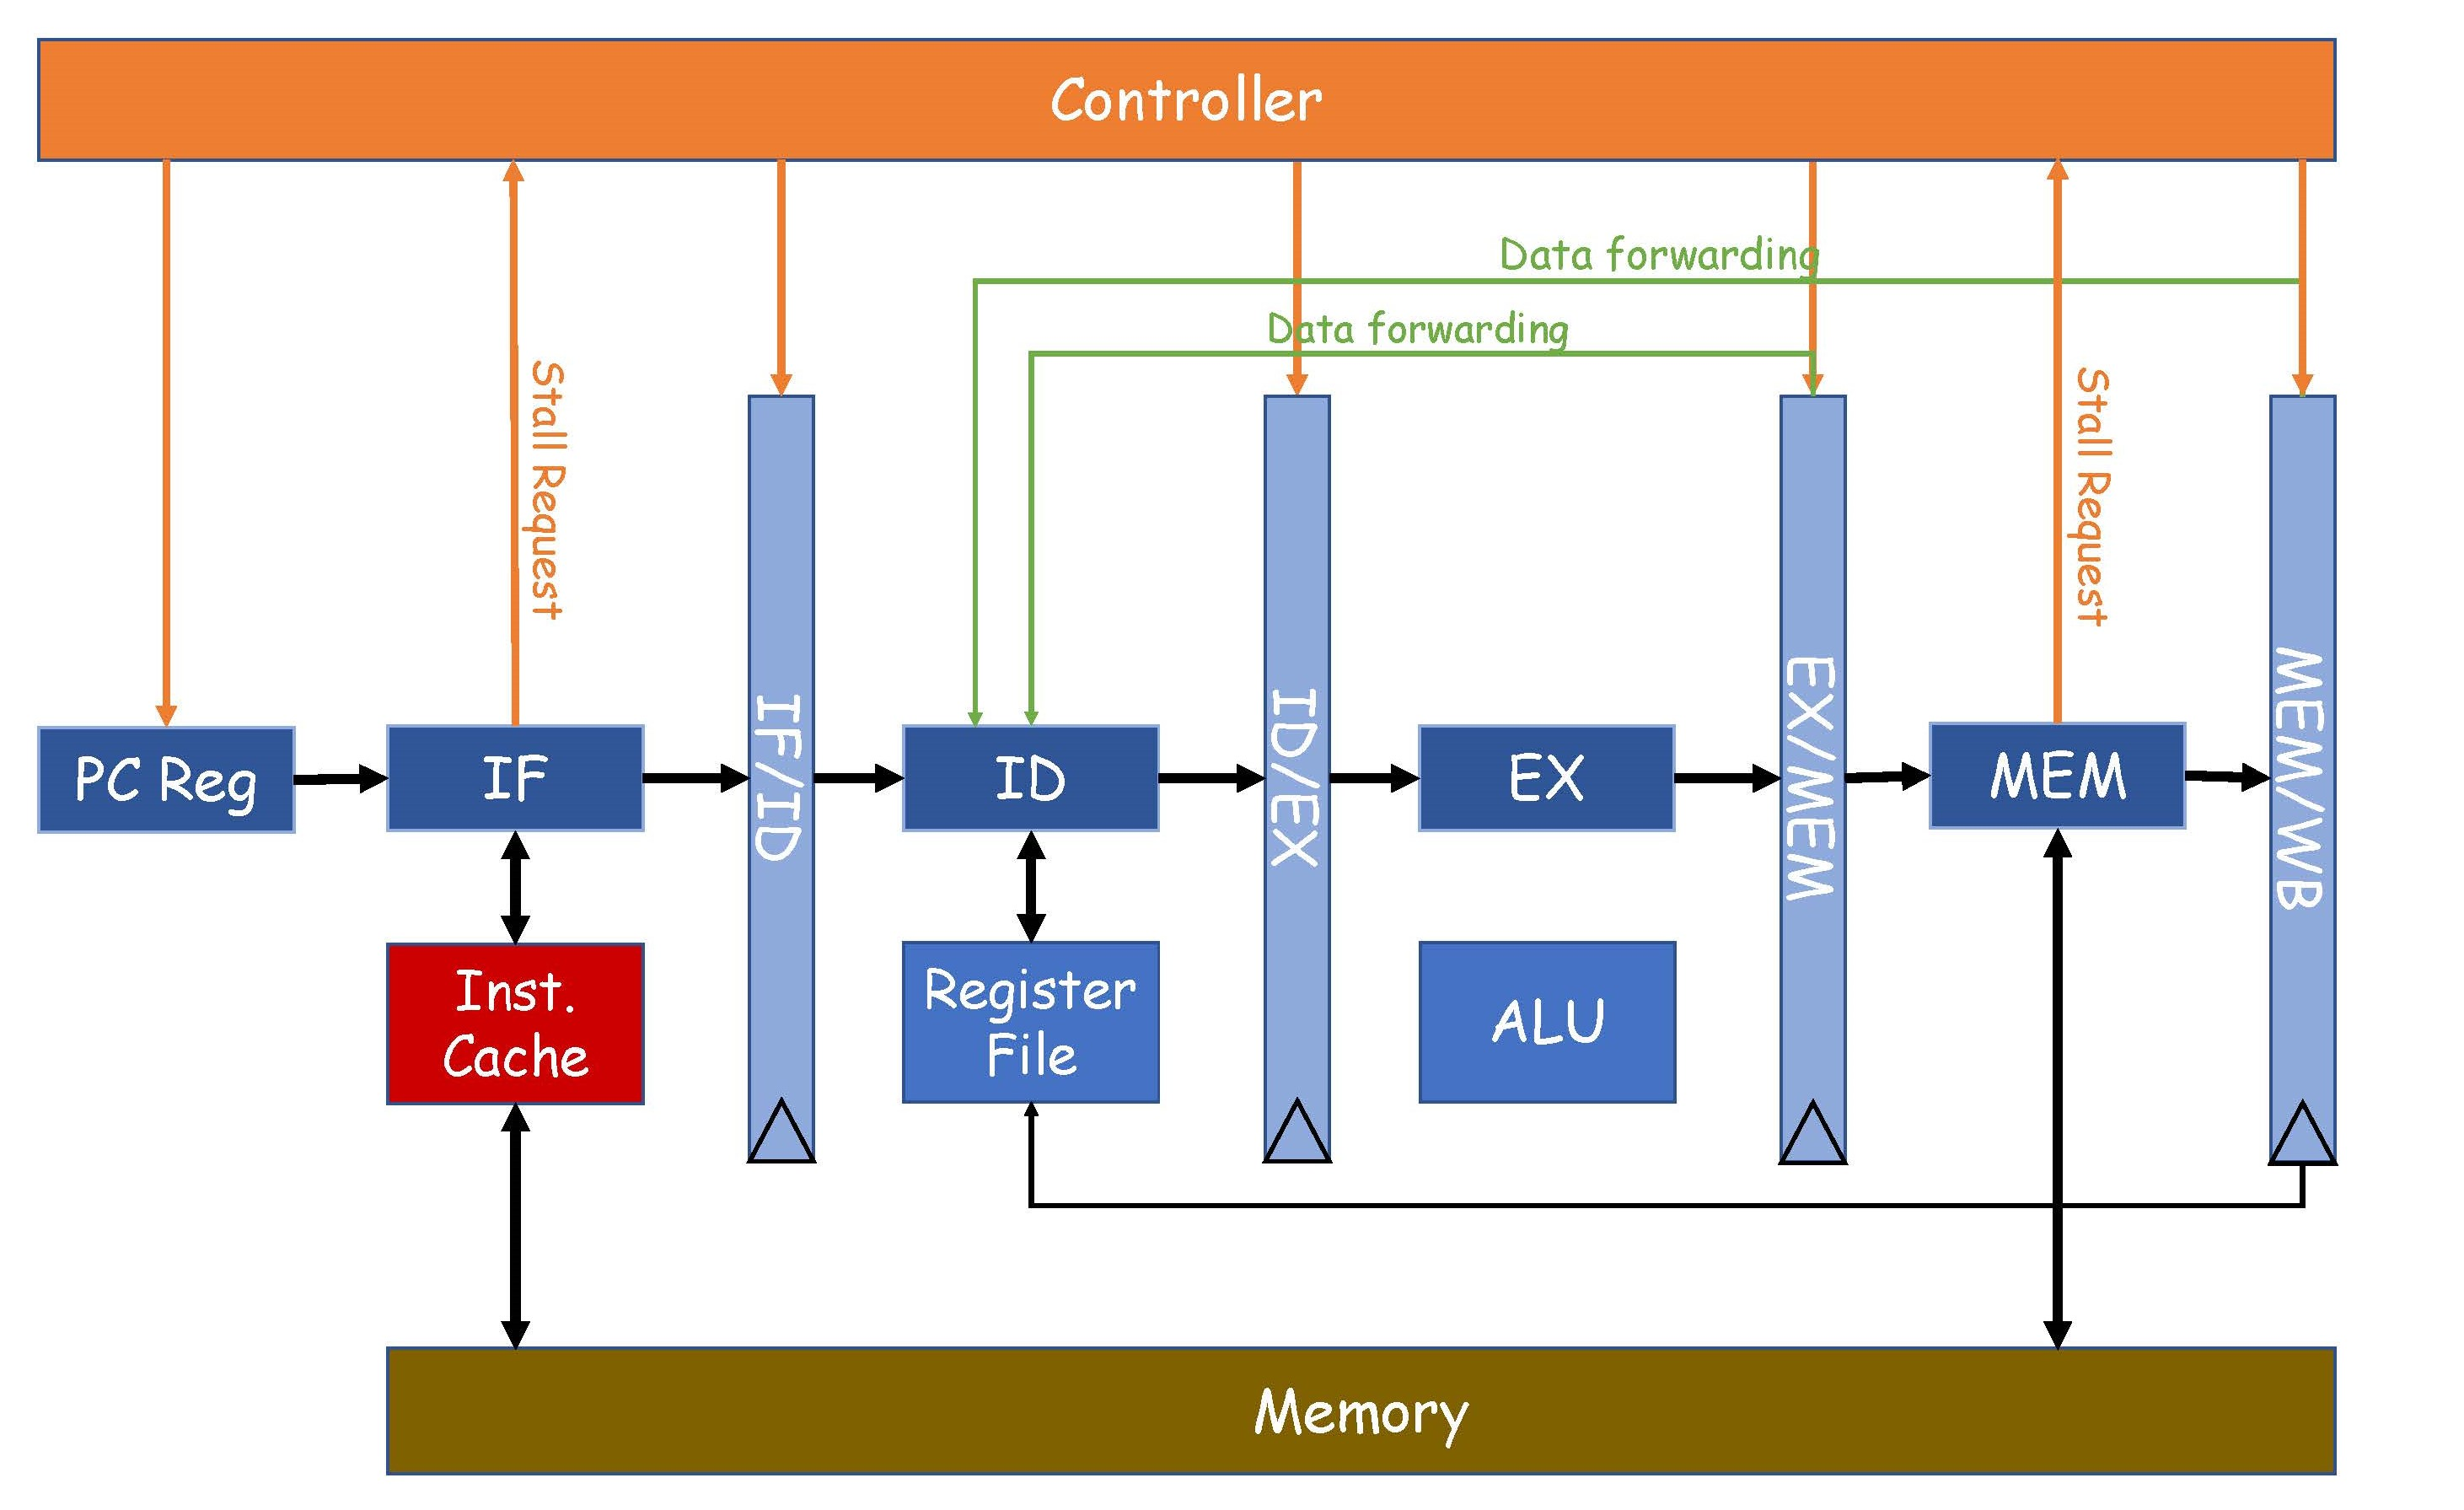
\includegraphics[scale=0.4]{datapath_diagram.jpg}
                \centering
                \caption*{\textbf{Figure 1}: Datapath Graph of the CPU}
            \end{figure}
        \section{Some remarks \& thoughts}
        \begin{enumerate}[label=(\arabic*)]
            \item Branch Prediction \\
                Branch Prediction requires calculating the target address in IF stage. However, a significant amount of delay will be introduced by implementing an adder in IF stage.\\
                Adding a \textbf{Branch Target Buffer(BTB)} resolves this problem. BTB records the target address for all \textit{taken} branches. Thus, the IF stage uses the current PC to index the BTB,
                if an entry is found, then the branch is predicted taken and the program uses the corresponding address as the next PC. 
            \item Overclocking \\
                Since I wrote the code with the principle of minimizing delay in mind, there is a positive $2ns$ WNS at $100MHz$. \\
                Overclocking to $250MHz$ still yields stable performance. \\
                At $250MHz$, testcase \textit{pi} takes $0.6$ seconds.
            \item Debugging \\
        \end{enumerate}
    \section{Conclusions}
        \begin{enumerate}[label=(\arabic*)]
            \item Smaller is faster. \\
                This is especially true when dealing with a not-so-good FPGA board. I tried
                \begin{itemize}\itemsep0em
                    \item adding an additional adder in the ID stage
                    \item making the cache bigger to hold more instruction
                    \item more sophisticated branch prediction schemes such as tournament predictor, predictor based on global history, etc.
                \end{itemize}
                Without any exception, the performance is undermined significantly.
                My final version is small(using only \~{}20\% of the board), but can be overclocked to achieve a pretty good performance.
            
        \end{enumerate}
    \section{References}
        \begin{enumerate}[label={[\arabic*]}]\itemsep0em
            \item 雷思磊. 自己动手写CPU, 电子工业出版社, 2014.
            \item John L. Hennessy, David A. Patterson, et al. \textit{Computer Architecture: A Quantitative Approach, Fifth Edition}, 2012.
        \end{enumerate}
\end{document}
